\chapter{Lecture 3 - Basics}
\section{Visual encoding}
Visual encoding means \emph{going from data to visual representations}. Encoding requires not only choosing a graph that is appropriate for the data at hand (its type and semantics), but also selecting the individual graphical elements and their properties.\par
There are two core graphical elements in a visualization: visual marks and visual channels. \emph{Marks} are basic geometric/graphical elements that depict items or links (a point, a line, a polygon, ...). \emph{Channels} are visual properties that control the appearance of marks (color, dimension, ...) and depict attributes.\par
They are the building blocks for analyzing visual encoding; even complex visual encoding can be broken down into components that can be analyzed in terms of their marks and channel structure. The effectiveness of marks and channels for encoding data depends on data types.

\begin{definition}[Marks]
    A mark is a basic graphical element, a geometric primitive. They are classified according to the number of spatial dimensions they require: 
    \begin{itemize} [noitemsep]
        \item 0-dim: points
        \item 1-dim: line, segments
        \item 2-dim: areas
        \item 3-dim: volumes
    \end{itemize}
\end{definition}

\begin{definition}[Channels]
    Visual channels are a way to control the appearance of marks and encode information about attributes, independent of the dimensionality of marks. Some main channels are:
    \begin{itemize}[noitemsep]
        \item spatial position: aligned, unaligned, depth, region ...
        \item color: hue, saturation, luminosity
        \item shape and texture
        \item slop and angle
        \item size: length(1D), area(2D), volume(3D)
    \end{itemize}
\end{definition}

Channels can be divided into 2 different categories, according to the two different sensor modalities on the human perceptual system: identity and magnitude channels.\par
\textbf{Identity} channels give information about what something is or where it is, like \textit{shape, color}.\par
\textbf{Magnitude} channels tell us how much of something there is, the \textit{length, area, saturation, size, ...}

\begin{definition}[Context]
    A contextual component can make a visualization much easier to interpret, such as legends, labels, annotations, and also grids, axes, reference lines, etc.
\end{definition}

\paragraph{Bar chart}
Bar chart encodes 2 attributes, a \emph{quantitative} one represented on the y-axis and a \emph{categorical} one represented on the x-axis.\par
Its typical mark is a line (bars, 1D marks). Two channels, one for vertical spatial position for the quantitative attribute and one for horizontal spatial position for the categorical attribute.

\paragraph{Scatterplot}
A scatterplot can encode multiple attributes. Its main mark is points (circles, 0D marks). It can have different channels: \textit{one} for vertical spatial position along the y-axis to represent a quantitative attribute; \textit{one} for horizontal spatial position along the x-axis for the second quantitative attribute; \textit{a third channel} could be color to represent a quantitative or qualitative attribute; a forth channel is the area of the points.

\section{Visual decoding}
Visual decoding means deconstructing a visual representation into its major units, and identifying the graphical elements \textit{(what are the visual marks and channels?)} and the mapping rules, i.e., the information that the graphical elements represent \textit{(What data items do the marks represent? What attribute do the channels represent?)}. It is useful for evaluating and redesigning visualizations.\par

\section{Expressiveness and Effectiveness}
Channels are not equal: the same data attribute encoded with two different visual channels will result in different information content on the users' side, after it has passed through the perceptual and cognitive pathways of the human visual system. \par
The use of marks and channels in visual design should be guided by the principles of \textbf{expressiveness and effectiveness}. There is a ranking of channels according to the type of data that is being visually encoded. Once you have identified the most important pieces of information in your data, you have to ensure they are encoded with the highest-ranked channels.

\begin{definition}[The Expressiveness Principle]
    The visual encoding should express all of, and only, the information that is present in the dataset attributes. Do not represent information and relationships that are not in the data, especially, do not use any color or position when the data does not encode any information.
\end{definition}

\textit{Ordered data} should be shown so that our visual system perceives them as ordered, by using \textit{magnitude channels.}\par
\textit{Unordered data} shouldn't be shown in a way that perceptually implies an ordering that does not exist, use \textit{identity channels}.

\begin{definition}[The Effectiveness Principle]
    The importance of the attribute should match the salience of the channel, i.e., its noticeability. Relevant information should be prioritized, then encoded with the most effective/accurate channels to be most noticeable. Decreasingly important attributes can be matched with less effective channels.
\end{definition}

\section{Channel rankings}
The ranking shows how effective the channels are at conveying different types of attributes.
\begin{figure}[htbp]
    \centering
    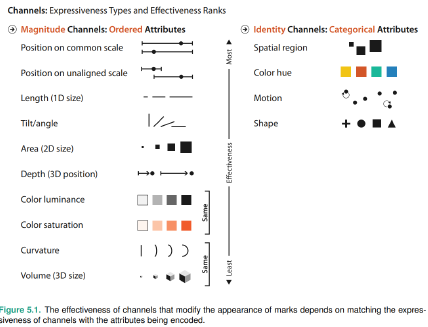
\includegraphics[width=\linewidth]{imgs/lecture3/3.4 channel rankings.png}
    \caption{A channel ranking}
    \label{fig:3.2}
\end{figure}

The fig~\ref{fig:3.4} shows one proposed channel ranking. As the figure shows, in both classifications, spatial channels appear at the top of the lists. The choice of which attributes to encode with position is the most central choice in visual encoding, as they will dominate a user's mental model.
\section{Visual representation, a counterexample}
\begin{figure}[htbp]
    \centering
    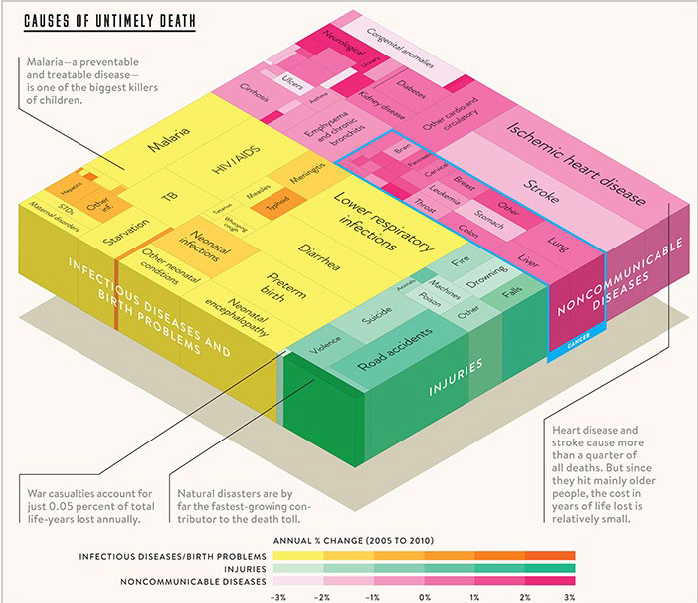
\includegraphics[width=0.5\linewidth]{imgs/lecture3/3.5 visual counterexample.png}
    \caption{A visual counterexample}
    \label{fig:3.5}
\end{figure}

The fig~\ref{fig:3.5} shows a visual representation of causes of death used in a debate. Where, each rectangle represents a death cause, the size of the rectangle represent years of life lost, the color represents the group of death, and the color intensity represents the change from one year to another.\par
It is a very complicated graph on a very complicated topic; some bad design choices made it less effective than it should be:
\begin{itemize}[noitemsep]
    \item the use of 3D projection is unnecessary, makes the perception of each rectangle much more difficult to comprehend.
    \item the area is not the best channel to represent quantities, also each rectangle has its own height and width, making the comparisons among causes much more difficult.
    \item Difficult in evaluating positive and negative changes by the use of color intensity
    \item Labels are too small to read
\end{itemize} 

\section{Channel effectiveness}
One would naturally ask how channel rankings are justified, and why some channels are better than others. Can all channels be used independently, or do they interfere with each other? We need a scientific answer.

\subsection{Accuracy}
\[S = I^n\]
S = perceived sensation; I = physical intensity; n = exponent.\par
The power law of Stevens models the response to sensory experience. Its exponent n ranged from the sublinear 0.5 for brightness to the superlinear 3.5 for electric current. \par
The sublinear phenomena are compressed, superlinear phenomena are magnified. Doubling the physical brightness results in a perception that is considerably less than twice as bright.\par
Humans can only perceive length as a very close match to the true value; all other visual channels are not perceived as accurately.

\begin{figure}[htbp]
    \centering
    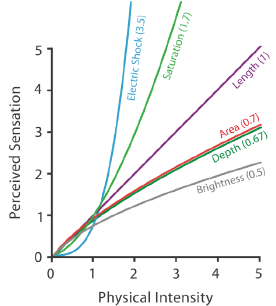
\includegraphics[width=0.3\linewidth]{imgs/lecture3/3.6 law of power.png}
    \caption{The power law of Stevens}
    \label{fig:3.4}
\end{figure}

\subsection{Discriminability}
Match the ranges: the number of different values that one needs to show for the attribute being encoded must not be greater than the number of bins available for the visual channel used to encode it. IF they do not match, one should use a different channel or aggregate the attributes into meaningful bins (highlights the most important one and aggregate all others under the same value, as others).
\subsection{Separability}
Channels may have dependencies and interactions with others, 
\begin{itemize}[noitemsep]
    \item from orthogonal and independent separable channels to the combined integral channels.
    \item Position and hue are completely separable.
    \item Size is not fully separable from color hue.
    \item Horizontal and Vertical size are an integral pair.
\end{itemize}   
\subsection{Pop-out}
Many visual channels provide visual pop-outs, where a distinct item stands out from many others immediately. It has an added value if the time it takes us to spot a different object does not depend on the number of distracting objects.
\begin{figure}[htbp]
    \centering
    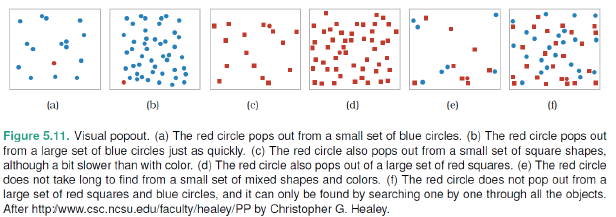
\includegraphics[width=0.5\linewidth]{imgs/lecture3/3.7 pop out.png}
    \caption{Visual pop-out}
    \label{fig:3.7}
\end{figure}
As a general rule, \textit{use pop-out for a single channel at a time}. Most pairs of channels do not support pop-out (except for the shape and color pair). Pop-out is not possible with 2 or more channels
\section{Relative Vs Absolute Judgments}
The human perceptual system is based on relative judgments, not absolute ones. The length difference we can detect is a percentage of the object's length.\par
When two objects are directly next to each other and aligned, we can make a much more precise judgment than when they are not.\par 
Our perception of color and luminance is completely contextual.

\begin{figure}[htbp]
    \centering

    \begin{subfigure}[b]{0.35\linewidth}
        \centering
        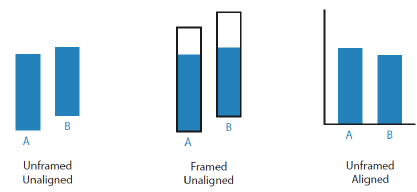
\includegraphics[width=\linewidth]{imgs/lecture3/3.8 relative judgement example 1.png}
        \caption{Are the 2 objects the same height?}
        \label{fig:3.8a}
    \end{subfigure}
    \hfill
    \begin{subfigure}[b]{0.35\linewidth}
        \centering
        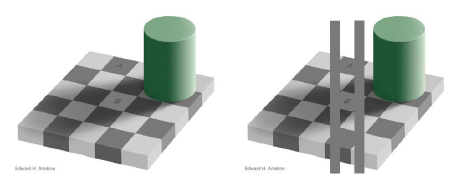
\includegraphics[width=\linewidth]{imgs/lecture3/3.8 relative judgement example 2.png}
        \caption{Are there different shades of gray?}
        \label{fig:3.8b}
    \end{subfigure}
    \hfill

    \caption{Relative judgment examples}
    \label{fig:3.8}
\end{figure}